\section{Tissue and Allele Heterogeneity}

\subsection{Variation among Human Tissues}

Performance varies across the 77 Human fixed-test tasks. For tuned TissuePMHC, the ten lowest task means have AUROC 0.6608, compared with 0.8136 over all tasks. The lowest individual task is brain--HLA-A*11:01 (0.6077), whereas the highest is breast--HLA-A*02:01 (0.9640). Table~\ref{tab:human-tissue-extremes} summarizes tissue means. These values are descriptive: each task contains 50 test pairs, and tissues differ in allele inventory and training coverage.

Figure~\ref{fig:tissue-colored-heterogeneity} shows every Human and Mouse task rather than only the tissue summaries. Point color has one meaning throughout the figure---target tissue---while navy horizontal marks show the corresponding tissue means. The spread within several tissues is comparable with the spread between tissue means, emphasizing that a tissue label does not determine performance independently of its MHC restriction and data inventory.

\begin{figure*}[t]
\centering
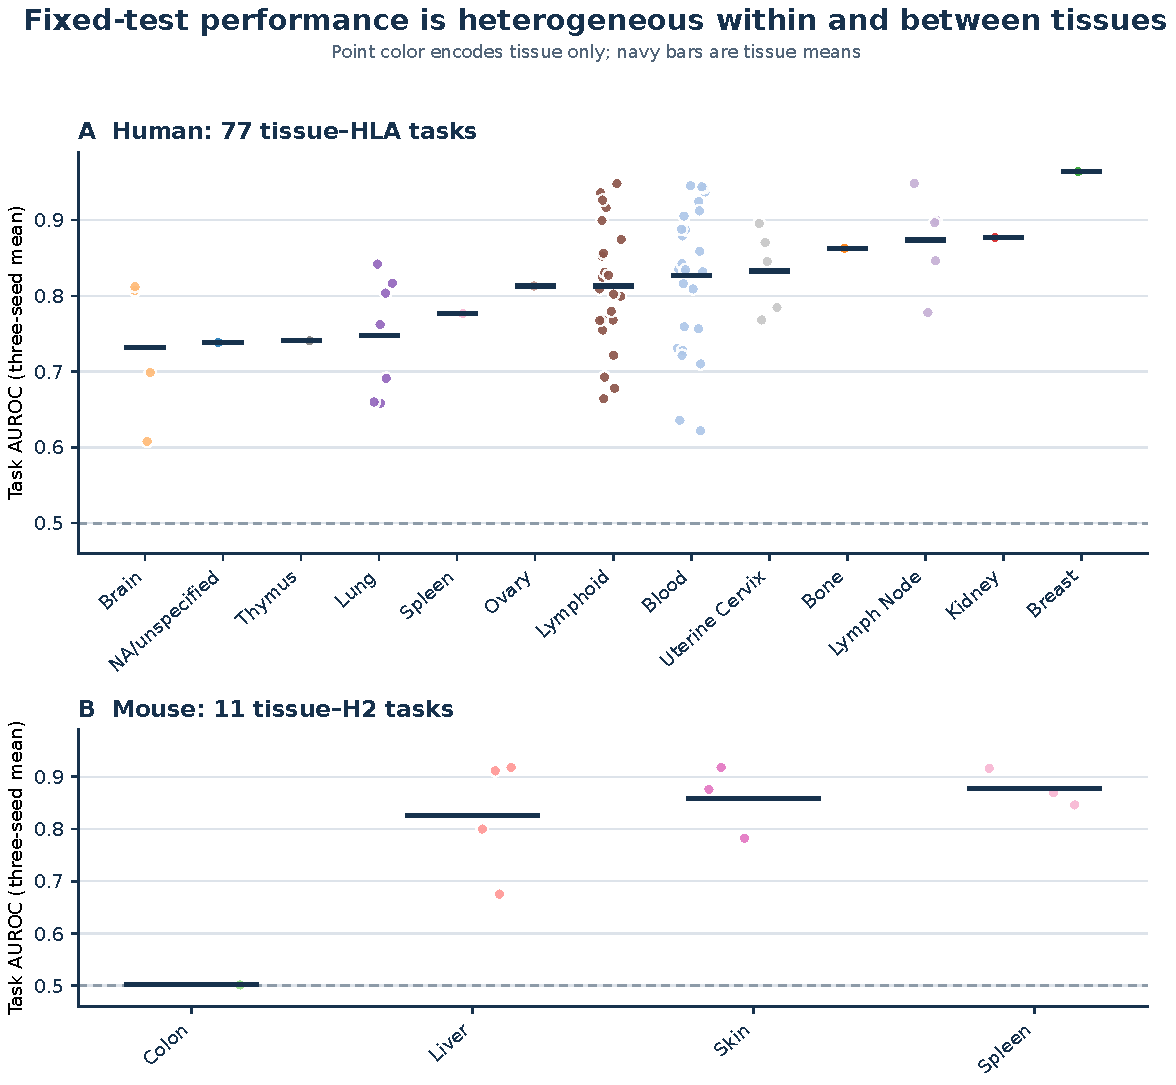
\includegraphics[width=0.90\textwidth]{figures/figure6_tissue_colored_heterogeneity.pdf}
\caption{Tissue-resolved fixed-test heterogeneity of tuned TissuePMHC on the occurrence-matched data. \textbf{A}, Three-seed mean AUROC for all 77 Human tissue--HLA tasks. \textbf{B}, Three-seed mean AUROC for all 11 Mouse tissue--H2 tasks. Each point is one task, point color encodes target tissue only, and the navy horizontal mark is the unweighted mean of the available tasks in that tissue. Tissues are ordered by their mean within each species. The dashed line at AUROC 0.5000 is a random-ranking reference, not an experimental observation. Differences among tissues are descriptive because tissue, MHC inventory, source study, peptide inventory, and training size are not controlled independently.}
\label{fig:tissue-colored-heterogeneity}
\end{figure*}

\begin{table*}[t]
\centering
\caption{Human tissue-level fixed-test performance of tuned TissuePMHC on the occurrence-matched data. The table describes heterogeneity rather than a controlled biological tissue ranking. Each of the 77 tasks is first averaged over the same three seeds; tissue means then weight the available HLA tasks equally. Task counts expose the unequal HLA inventory across tissues. Tissues are ordered by AUROC from top to bottom in the left block and then the right block; the blank source label is reported as ``NA/unspecified.''}
\label{tab:human-tissue-extremes}
\footnotesize
\begin{tabularx}{\textwidth}{>{\raggedright\arraybackslash}Xrrr>{\raggedright\arraybackslash}Xrrr}
\toprule
Tissue & Tasks & AUROC & AUPRC & Tissue & Tasks & AUROC & AUPRC \\
\midrule
Brain & 4 & 0.7314 & 0.7393 & Blood & 26 & 0.8265 & 0.8345 \\
NA/unspecified & 1 & 0.7384 & 0.7261 & Uterine cervix & 5 & 0.8328 & 0.8262 \\
Thymus & 1 & 0.7407 & 0.7548 & Bone & 1 & 0.8627 & 0.8762 \\
Lung & 7 & 0.7476 & 0.7417 & Lymph node & 5 & 0.8737 & 0.8583 \\
Spleen & 1 & 0.7765 & 0.7834 & Kidney & 1 & 0.8769 & 0.9003 \\
Lymphoid & 23 & 0.8129 & 0.8032 & Breast & 1 & 0.9640 & 0.9657 \\
Ovary & 1 & 0.8129 & 0.8200 & & & & \\
\bottomrule
\end{tabularx}
\end{table*}

The broad range should not be interpreted as a biological tissue hierarchy. Tissue identity is confounded with the available HLA restrictions, source studies, peptide inventory, and training-set size.

\subsection{Variation among Mouse Tissue--H2 Tasks}

Tuned Mouse TissuePMHC has task-macro AUROC 0.8194, with task means spanning 0.5016--0.9180 (Table~\ref{tab:mouse-task-detail-new}). H2-Db is the weakest descriptive restriction group (0.5885), while H2-Kk and H2-Kd reach 0.9011 and 0.9018. Each restriction occurs in a different tissue subset, so these are not controlled H2 effects.

\begin{table*}[t]
\centering
\caption{Mouse heterogeneity of tuned TissuePMHC on the occurrence-matched fixed test. \textbf{A}, All 11 tissue--H2 task values, each averaged over the same three seeds and ordered by AUROC. \textbf{B}, Descriptive H2-restriction means formed after the seed-level task averages, with tasks weighted equally. Task counts expose the available tissue inventory. The table describes internal heterogeneity and cannot isolate tissue or H2 effects because the represented contexts differ.}
\label{tab:mouse-task-detail-new}
\footnotesize
\begin{minipage}[t]{0.57\textwidth}
\textbf{A. Tissue--H2 tasks}\par\smallskip
\begin{tabularx}{\linewidth}{>{\raggedright\arraybackslash}Xlrr}
\toprule
Tissue & H2 & AUROC & AUPRC \\
\midrule
Colon & H2-Db & 0.5016 & 0.5025 \\
Liver & H2-Db & 0.6754 & 0.6695 \\
Skin & H2-Kb & 0.7821 & 0.8124 \\
Liver & H2-Kb & 0.7999 & 0.8186 \\
Spleen & H2-Kb & 0.8461 & 0.8524 \\
Spleen & H2-Kd & 0.8693 & 0.8676 \\
Skin & H2-Kk & 0.8760 & 0.8920 \\
Liver & H2-Kk & 0.9113 & 0.9126 \\
Spleen & H2-Kk & 0.9161 & 0.9220 \\
Liver & H2-Kd & 0.9180 & 0.9137 \\
Skin & H2-Kd & 0.9180 & 0.9440 \\
\bottomrule
\end{tabularx}
\end{minipage}
\hfill
\begin{minipage}[t]{0.35\textwidth}
\textbf{B. H2 restriction groups}\par\smallskip
\centering
\begin{tabular}{lrrr}
\toprule
H2 restriction & Tasks & AUROC & AUPRC \\
\midrule
H2-Db & 2 & 0.5885 & 0.5860 \\
H2-Kb & 3 & 0.8094 & 0.8278 \\
H2-Kd & 3 & 0.9018 & 0.9085 \\
H2-Kk & 3 & 0.9011 & 0.9089 \\
\bottomrule
\end{tabular}
\end{minipage}
\end{table*}

The five lowest Mouse task AUROCs average 0.7210. With only 50 test pairs per task, individual task estimates are sensitive to a small number of pair reversals.

\subsection{Task-wise Effect of Training-only Tuning}

Figure~\ref{fig:tuning-delta-by-species} compares the selected tuned TissuePMHC configuration with the otherwise corresponding untuned multi-kernel model on exactly matched fixed-test tasks. In Human, the mean task-wise AUROC change is +0.0054 (10,000-task-bootstrap 95\% interval, $[+0.0011,+0.0098]$); 54 of 77 tasks improve and 23 decline. In Mouse, the mean change is +0.0489 ($[+0.0300,+0.0680]$); 10 of 11 tasks improve and one declines. Two-sided paired Wilcoxon signed-rank tests give Holm-adjusted $p=0.0060$ for Human and $p=0.0039$ for Mouse. These calculations establish consistency across the fixed-test task inventory, not patient-level or external-cohort significance, because tasks can share tissues, MHC restrictions, proteins, and source studies.

\begin{figure*}[t]
\centering
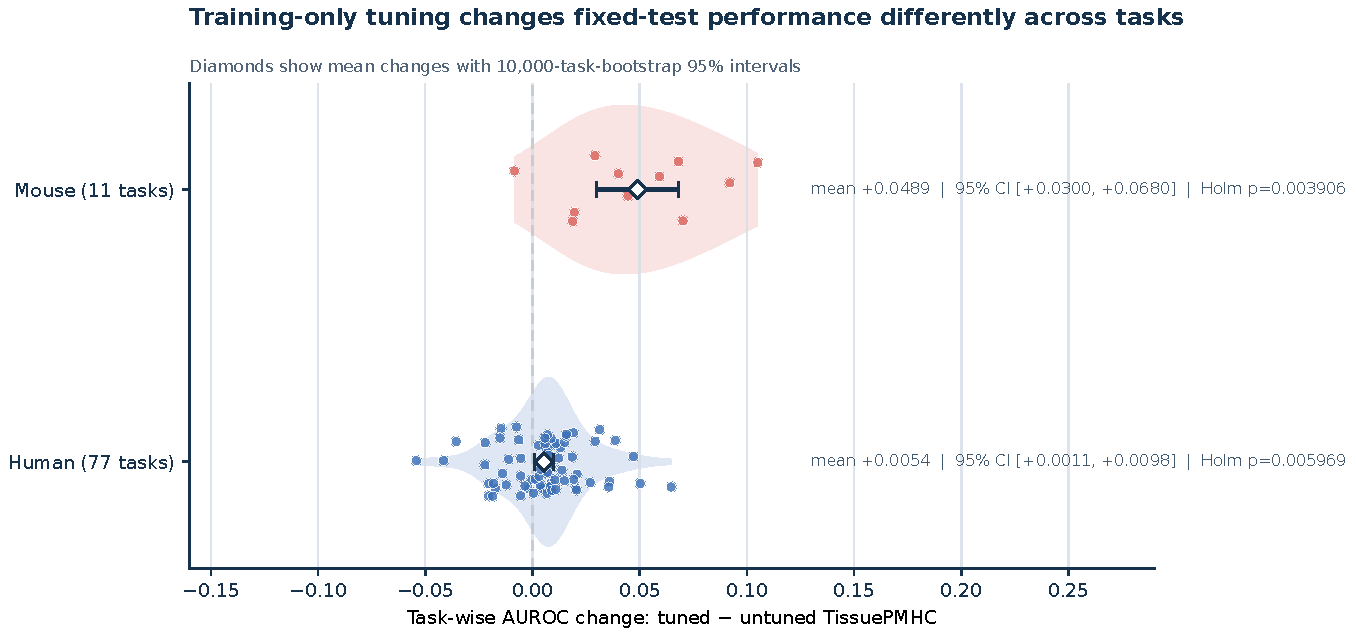
\includegraphics[width=0.90\textwidth]{figures/figure7_tuned_vs_untuned_task_deltas.pdf}
\caption{Task-wise change in fixed-test AUROC after training-only hyperparameter tuning. Each point is the difference between tuned and untuned TissuePMHC after first averaging the same task over seeds; positive values favor the tuned configuration. Open diamonds show the mean change, and horizontal bars show 95\% intervals from 10,000 bootstrap resamples of complete tasks. Two-sided paired Wilcoxon signed-rank tests were performed separately for Human and Mouse, then adjusted together by Holm's method (Human: 77 tasks, mean +0.0054, 54 improved, adjusted $p=0.0060$; Mouse: 11 tasks, mean +0.0489, 10 improved, adjusted $p=0.0039$). The intervals and tests describe this internal fixed-test task inventory and are not biological-replicate or cohort-level inference.}
\label{fig:tuning-delta-by-species}
\end{figure*}

\subsection{Human HLA-level Heterogeneity}

Human performance is heterogeneous across HLA loci and four-digit allele typings. For tuned TissuePMHC, HLA-A, HLA-B, and HLA-C task-macro AUROCs are 0.7778, 0.8032, and 0.8788, respectively. Table~\ref{tab:human-hla-locus} reports the five lowest and five highest four-digit typings, but the loci cover different tissues and training inventories.

This display differs deliberately from the Mouse H2 summary: Human contains 29 retained four-digit HLA typings, so an extreme-value overview is used, whereas Mouse contains only four H2 restrictions and Table~\ref{tab:mouse-task-detail-new} reports all four. Neither display supports a controlled cross-species allele ranking.

\begin{center}
\begin{minipage}{\columnwidth}
\captionof{table}{Lowest and highest Human four-digit HLA typings by mean fixed-test AUROC of tuned TissuePMHC. Each task is first averaged over the same three seeds on the occurrence-matched fixed test; allele means then weight the represented tissue--HLA tasks equally. Typings are selected solely by AUROC, five from each tail, while AUPRC is shown as a secondary metric. Task counts expose unequal tissue coverage, so the table is a descriptive extreme-value summary rather than a controlled allele ranking.}
\label{tab:human-hla-locus}
\centering
\scriptsize
\begin{tabularx}{\columnwidth}{lXrrr}
\toprule
Group & HLA typing & Tasks & AUROC & AUPRC \\
\midrule
Lowest & HLA-A*29:02 & 2 & 0.6500 & 0.6404 \\
Lowest & HLA-A*11:01 & 3 & 0.6550 & 0.6468 \\
Lowest & HLA-B*44:03 & 3 & 0.7036 & 0.6999 \\
Lowest & HLA-B*49:01 & 2 & 0.7296 & 0.7105 \\
Lowest & HLA-B*40:02 & 3 & 0.7442 & 0.7178 \\
\midrule
Highest & HLA-C*16:01 & 2 & 0.9351 & 0.9312 \\
Highest & HLA-B*27:09 & 2 & 0.9143 & 0.9176 \\
Highest & HLA-B*27:05 & 2 & 0.9120 & 0.9082 \\
Highest & HLA-C*14:02 & 2 & 0.9119 & 0.9177 \\
Highest & HLA-C*05:01 & 3 & 0.9010 & 0.8968 \\
\bottomrule
\end{tabularx}
\end{minipage}
\end{center}

Errors are enriched in several low-performing HLA-A and HLA-B tasks, but no single locus or tissue accounts for all difficult cases. The fixed internal test does not separate biological heterogeneity from study, coverage, or sampling effects.
